\section{Background and Motivation}
\label{sec:background}

\begin{figure}[t]
   \centering
   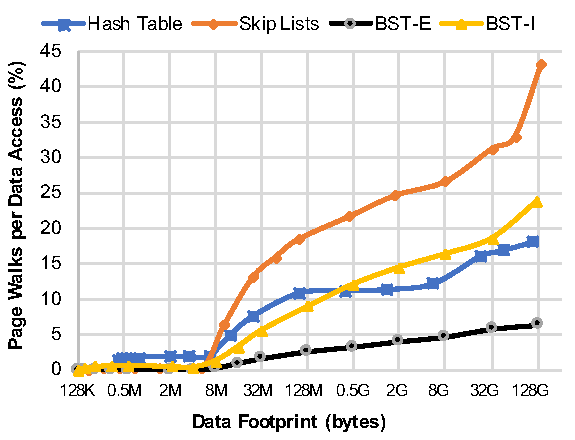
\includegraphics[width=1.0\columnwidth]{graphs/pagewalks.pdf}
   \caption{Frequency of page walks as a function of memory size.}
   \label{fig:pagewalks}
\end{figure}


\begin{table*}[]
\centering
\caption{Comparison of SpryVM with previous approaches for reducing virtual memory overhead.}
\label{table:vms}
\begin{tabular}{
>{\columncolor[HTML]{FFFFFF}}l |
>{\columncolor[HTML]{FFFFFF}}c |
>{\columncolor[HTML]{FFFFFF}}c |
>{\columncolor[HTML]{FFFFFF}}c |
>{\columncolor[HTML]{FFFFFF}}c |}
\cline{2-5}
\multicolumn{1}{c|}{\cellcolor[HTML]{FFFFFF}}                           & Programmability  & Performance and Efficiency & Flexibility & Safety and Security \\ \hline
\multicolumn{1}{|l|}{\cellcolor[HTML]{FFFFFF}Multi-page mappings~\cite{pham:colt, pham:increasing}}       & \cmark              & \xmark                          & \cmark           & \cmark      \\ \hline
\multicolumn{1}{|l|}{\cellcolor[HTML]{FFFFFF}Transparent Huge Pages~\cite{transparenthugepages}}    & \cmark               & \xmark                          & \cmark           & \cmark      \\ \hline
\multicolumn{1}{|l|}{\cellcolor[HTML]{FFFFFF}libhugetlbfs~\cite{lighugetlbfs}}              & \xmark                & \xmark                          & \cmark           & \cmark      \\ \hline
\multicolumn{1}{|l|}{\cellcolor[HTML]{FFFFFF}Direct Segments~\cite{basu:efficient}}           & \xmark              & \cmark                          & \xmark           & \cmark      \\ \hline
\multicolumn{1}{|l|}{\cellcolor[HTML]{FFFFFF}Redundant Memory Mappings~\cite{karakostas:redundant}}  & \cmark             & \xmark                          & \xmark           & \cmark      \\ \hline
\multicolumn{1}{|l|}{\cellcolor[HTML]{FFFFFF}Direct-mapped Mappings~\cite{picorel:near-memory, haria:devirtualizing}}         & \cmark       & \cmark                          & \xmark           & \cmark      \\ \hline
\multicolumn{1}{|l|}{\cellcolor[HTML]{FFFFFF}SpryVM}                    & \cmark                       & \cmark               & \cmark           & \cmark      \\ \hline
\end{tabular}
\end{table*}

\subsection{Goals for VM in Heterogeneous Systems}
When buiding VM support for accelerators, it is important to identify
design goals for the its operation. Like prior work
\cite{haria:devirtualizing}, we identify the following as key goals in
our design:

\begin{itemize}
        \item \textbf{Programmability.} The widespread adoption of
          accelerators rests on the usability of and familiarity of
          their programming models. Unified virtual memory between
          CPUs and accelerators are one way of achieving this in a
          manner that simplifies data sharing, eliminating the need
          for hand-managed data copying and marshaling. Ideally, we
          wish to preserve all the benefits typically associated with
          VM like memory protection and isolation, and flexibility of
          sharing parts of the address space among processes, in a
          manner that is transparent and familiar to programmers.

        \item \textbf{Flexibility.} Traditional VM imposes no
          restrictions on virtual-to-physical page mapping
          relationships. This is valuable to support any level of
          system memory fragmentation, application multi-tenancy,
          memory allocation strategies transparent to programmers, as
          well as the integration of features such as demand-paging
          and copy-on-write (CoW). We wish to continue supporting this
          flexibility.

        \item \textbf{Safety and Security.} Direct access to physical
          memory is generally not acceptable nor desirable. Such
          memory management approaches cannot prevent malicious or
          erroneous memory accesses and prohibits sharing accelerators
          across different processes with proper
          isolation~\cite{haria:devirtualizing}. Furthermore, the
          entropy in address mapping must be as high as possible to
          reduce the vulnerability to security attacks.

        \item \textbf{Performance and Efficiency.} Crucially, all the
          goals listed thus far must be achievable without excessive
          performance or area overheads in hardware. In other words,
          address translation, the central mechanism on which VM's
          benefits rest, must provide near-zero performance overheads
          regardless of application working set and locality patterns,
          and must do so under tight area and power constraints. In
          the context of accelerators, the area and power budgets are
          even tighter because custom hardware is only integrated if
          it provides large performance benefits with minimal
          resources.


\end{itemize}


\subsection{Shortcomings of modern MMU Hardware}
Today's systems employ ever increasing mamory sizes, particularly in the server domain where large portions of data are often kept in memory for latency reasons. Such a trend, together with the slowdown in silicon density scaling, forces the system designers to adopt the scale-out approach not only to compute resources, but also to memory resources. This has two major implications on virtual memory: reduced TLB effectiveness and increased page walk latency. 

\subsubsection{TLB inefficiencies}
As the memory capacity keeps increasing, TLB hit ratios decrease sharply~\cite{basu:efficient} resulting in significantly higher frequency of page walks. This effect is further exacerbated by increasingly irregular access patterns of modern big data applications that lack spatial and temporal locality~\cite{haria:devirtualizing}. In response, modern systems have embraced larger and more complex TLB hierarchies in an effort to increase the TLB reach. However, increasing the TLB size beyond a few dozen entries provides diminishing returns when accessing hundreds of gigabytes of memory, especially in the absence of spatial and temporal locality. Figure~\ref{fig:pagewalks} shows the number of page walks per memory access as a function of the memory footprint for a set of data traversal benchmarks running on an Intel Broadwell chip (for methodology details, please refer to Section~{sec:methodology}). The first thing to note that even large and deep TLB hierchies with >1.5K TLB entries cannot deal with irregular traversals of large datasets. The second thing to note is that the frequency of page walks sharply increases with the size of the data. This result corroborates a prior study on TLB ineffetiveness~\cite{basu:efficient}, which also observed similar trends with larger pages sizes. While large pages are highly effective in reducing translation overheads, they may not be suitable for accelerators, and ultimately do not solve the problem as memory continues to scale~\cite{basu:efficient}.	

The area and power overheads of the translation hardware become particularly concerning and impractical in heterogeneous systems with a large number of tiny, highly customized accelerators~\cite{haria:devirtualizing}, where the overheads of the translation hardware can greatly surpass the power and area of the rest of the functional parts of the accelerator. Given the increasing gap between the memory growth and practical TLB capacity growth~\cite{gandhi:badgertrap}, the TLB performance is certainly not on a promising trajectory.

The underlying reason for poor TLB performance is that TBLs cache translation on the execution side. Because of that, every execution unit (be it a core or accelerator) must have a TLB unit, each of which caches translations that cover the entire physical memory. This becomes impractical, because the total amount of translation hardware in the system grows linearly with the number of execution units, as well as ineffective, because the memory growth makes each of the TLB units incapable of achieving sufficient hit ratios. In contrast, if we were able to design a system where TLBs would act as memory-side translation caches, each serving one memory partition, then the number of TLBs would not depend on the number of execution units. More importantly, such TLBs would only need to cover a fraction of the dataset, which would significantly increase their TLB hit ratios, as per Figure~\ref{fig:pagewalks}.

\subsubsection{Increasing page walk latency}
Modern CPUs heavily depend on MMU caches to reduce the number of memory access per page walk. However, even with perfect MMU caches, page walks in the best case comprise of one access to a random memory element. As the average distance between compute and memory elements keeps increasing, the latency of page walks increases proportionately. The situation is more concerning for heterogeneous systems, because the accelerators may not have the sufficient resources to implement large enough MMU caches and may require many more memory references per page walk. 

\subsection{Prior Approaches}

This part and Table~\ref{table:vms} overviews all prior work in memory management mechanism in terms of the aforesaid four goals presented before.

\noindent\textbf{Multi-page mappings.} Several studies exploited
the contiguity naturally generated by the buddy allocator and the
memory compactor. CoLT~\cite{pham:colt} and clustered~\cite{pham:increasing} TLBs coalesce 4-8 page translations into a single TLB entry, as long as their physical locations are contiguous. Although the TLB reach improves, it is still unable to cover the entirety of a large memory system of tens or hundreds of GBs~\cite{gandhi:range}, requiring large, deep, and power-hungry TLB hierarchies to cover all the memory.

\noindent\textbf{Huge pages.} The most common approach to increase the TLB reach is the introduction of larger page sizes by using Transparent Huge Pages (THP)~\cite{transparenthugepages} and libhugetlbfs~\cite{lighugetlbfs}. In commercial x86 and ARM architectures, 2MB and 1GB pages are supported in addition to the traditional 4KB page size. Unfortunately, the OS can only allocate huge pages when the available physical memory is size-aligned and contiguous, which is not possible when the system is under memory pressure. Furthermore, supporting multiple page sizes heavily increases the TLB hardware complexity, making huge pages unsuitable for area- and power-efficient accelerators.

\noindent\textbf{Segments.} More innovative ways of improving TLB coverage is the usage of variable-size segments instead of fixed page-based translations~\cite{karakostas:redundant, park:hybrid, basu:efficient}. Unfortunately, the effectiveness of these techniques relies on heavy changes to the OS's allocation path with at-allocation contiguity generation (i.e., eager paging). Furthermore, direct segments require applications to explicitly allocate a segment at startup, while redundant memory mappings (RMMs)~\cite{karakostas:redundant} requires highly associative power-hungry TLBs, both very unattractive from the programmability and hardware-efficiency perspectives.

\noindent\textbf{Direct-mapped mappings.} These techniques deliver almost near-zero overhead as they completely overlap translation with data fetch. Unfortunately, these techniques severely restrict the OS's memory allocation mechanism by either using identify mapping~\cite{haria:devirtualizing} or direct-mapped page-level allocation~\cite{picorel:near-memory}. The allocation restrictions limit the performance of such techniques with fragmented and application multi-tenancy scenarios, and complicate traditional OS mechanisms such as copy-on-write (COW) and the widely used fork system call optimization. Furthermore, these approaches drastically reduce the amount of entropy in address mapping, making the system more vulnerable to security attacks.


\javier{Points to come across:

\begin{itemize}
  \item SW trend: Servers workloads are keeping their datasets memory resident; HW trend: Due to slowdown in silicon density and efficiency, computer system are integrating custom logic (accelerators).
  \item Explain the programmability benefits of pointer-is-a-pointer AND flexible VM system (e.g., demand paging, COW) of a conventional translation mechanism.
  \item TLB Reach Problem: Explain that a conventional translation mechanism is not effective for accelerators because (1) it relies on deep cache and TLB hierarchies and (2) data reuse, to bridge the gap between computation speed and memory capacity. However, accelerators primarily exploit parallel access with proximity to memory, and not reuse and deep cache hierarchies. Furthermore, accelerator are custom and hence silicon optimized, hence the available budget for translation hardware is limited. I think we can just cite prior work on TLB miss rates for in-memory workloads.   
  \item TLB Penalty Problem: Explain that compute and memory are scaling-out due to the slowdown in silicon scaling and efficiency, hence TLB misses (page walks) become more costly. We can show something similar to Figure 1 here.
\end{itemize}


}

